\documentclass[svgnames,11pt]{beamer}
\input{/home/tof/Documents/Cozy/latex-include/preambule_commun.tex}
\input{/home/tof/Documents/Cozy/latex-include/preambule_beamer.tex}
%\usepackage{pgfpages} \setbeameroption{show notes on second screen=left}
\author[]{Christophe Viroulaud}
\title{Pierre Feuille Ciseaux \\Fonction}
\date{\framebox{\textbf{Lang 05}}}
%\logo{}
\institute{Première - NSI}
%DODO faire plus de python tutor dès le début <-- comment l'afficher au tableau? faire une simul dans slides?
%DODO insister sur structure d'un fichier: fonction au début, prog principal
\begin{document}
\begin{frame}
\titlepage
\end{frame}
\begin{frame}
    \frametitle{}

    Le jeu \emph{pierre - feuille - ciseaux} est un jeu effectué avec les mains et opposant deux joueurs.
    \begin{center}
    \centering
    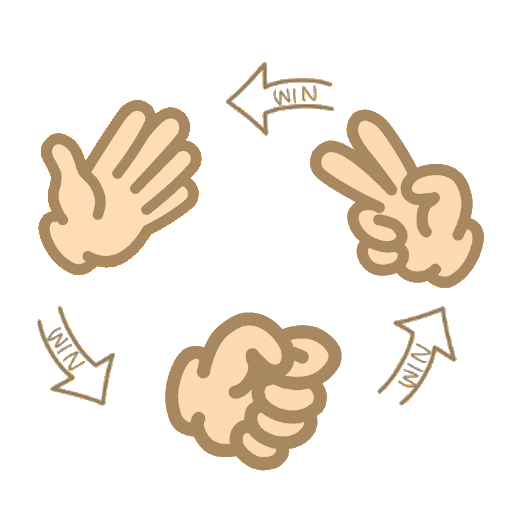
\includegraphics[width=5cm]{ressources/pfc.png}
    \captionof{figure}{Chaque flèche va dans le sens du gagnant.}
    \label{IMG}
    \end{center}
\end{frame}
\begin{frame}
    \frametitle{}
\begin{center}
    \begin{tabular}{ccc}
        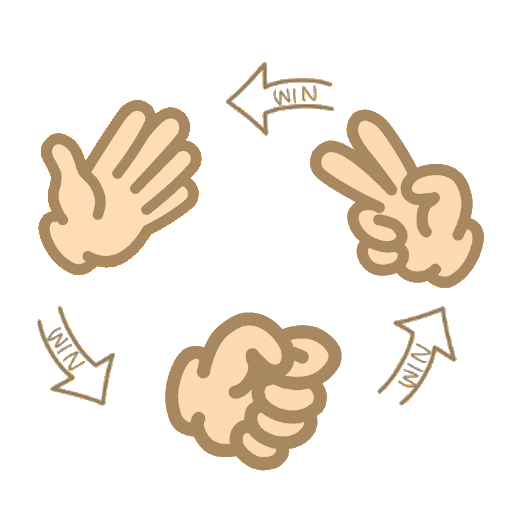
\includegraphics[width=3cm]{ressources/pfc.png}
        &
        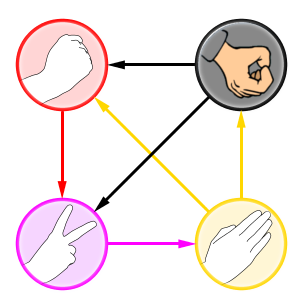
\includegraphics[width=3cm]{ressources/pfcp.png}
        &
        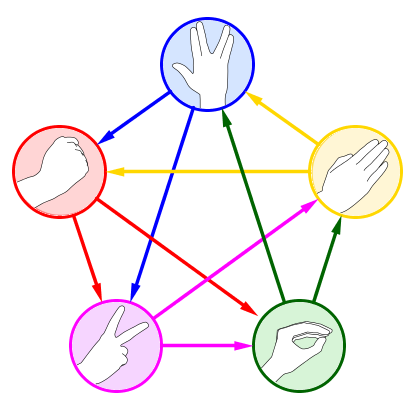
\includegraphics[width=3cm]{ressources/pfcls.png}
    \end{tabular}
    \captionof{figure}{Il existe plusieurs variantes de ce jeu.}
\end{center}
    \begin{center}
        \begin{framed}
            \centering Quel concept mettre en place pour implémenter le jeu de manière lisible?
        \end{framed}
    \end{center}

\end{frame}
\section{Notion de fonction}
\subsection{Fonction mathématique}
\begin{frame}
    \frametitle{Fonction mathématique}
    On peut voir une fonction comme une boîte noire qui:
    \begin{itemize}
        \item accepte éventuellement un \textbf{paramètre},
        \item \textbf{renvoie} une valeur.
    \end{itemize}
$$f(x)=x^3$$
    \begin{center}
        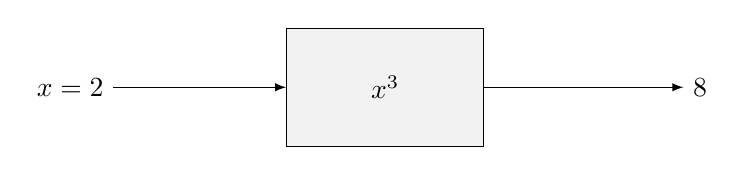
\begin{tikzpicture}
            \node(x) at (-4,0) {$x=2$};
            \node[draw,fill=gray!10,minimum width=2.5cm,minimum height=1.5cm] (f) at (0,0) {$x^3$};
            \node(res) at (4,0) {8};
            
            \draw[->,>=latex] (x) -- (f);
            \draw[->,>=latex] (f) -- (res);
            \end{tikzpicture}
            \captionof{figure}{paramètre: $x=2$; valeur renvoyée: 8}
    \end{center}

\end{frame}
\subsection{Fonction en programmation}
\begin{frame}[fragile]
    \frametitle{Fonction en programmation}

\begin{center}
\begin{lstlisting}[language=Python , basicstyle=\ttfamily\small, xleftmargin=2em, xrightmargin=2em]
def cube(x):
    valeur = x**3
    return valeur
\end{lstlisting}
\captionof{code}{Création d'une fonction}
\label{CODE}
\end{center}

\end{frame}
\begin{frame}[fragile]
    \frametitle{}

    \begin{center}
        \begin{tikzpicture}
            \node(x) at (0,0) {\begin{lstlisting}[language=Python , basicstyle=\ttfamily\small, backgroundcolor={},rulecolor=\color{white},numbers=none]
def cube(x):
    valeur = x**3
    return valeur
\end{lstlisting}};
\node (creer) at(-3,2){créer};
\draw[->,>=latex] (creer.south) -- (-1.5,0.5);
\node (nom) at(-0.5,2){nommer};
\draw[->,>=latex] (nom.south) -- (-0.5,0.5);
\node (parametre) at(3,2){paramètre};
\draw[->,>=latex] (parametre.south) -- (0.1,0.5);
\node (renvoie) at(0,-2){renvoyer};
\draw[->,>=latex] (renvoie.north) -- (0,-0.5);
\end{tikzpicture}
\captionof{figure}{Création de la \emph{boîte}.}
    \end{center}

\end{frame}
\begin{frame}[fragile]
    \frametitle{}

    \begin{center}
    \begin{lstlisting}[language=Python , basicstyle=\ttfamily\small, xleftmargin=2em, xrightmargin=2em]
>>> cube(2)
8
\end{lstlisting}
    \captionof{code}{Appel de la fonction}
    \label{CODE}
    \end{center}

\end{frame}
\section{Pierre feuille ciseaux}
\subsection{Création de la fonction}
\begin{frame}
    \frametitle{Création de la fonction}

Pour jouer contre l'utilisateur, la machine doit choisir au hasard parmi les propositions: \emph{pierre, feuille, ciseaux}.
\begin{activite}
Écrire la fonction \textbf{\texttt{choix\_machine()}} qui renvoie aléatoirement un des trois mots: \emph{pierre, feuille, ciseaux}.
\end{activite}

\end{frame}
\begin{frame}[fragile]
    \frametitle{Correction}

\begin{center}
\begin{lstlisting}[language=Python , basicstyle=\ttfamily\small, xleftmargin=2em, xrightmargin=2em]
def choix_machine():
    valeur = randint(1, 3)
    if valeur == 1:
        choix = "pierre"
    elif valeur == 2:
        choix = "feuille"
    else:
        choix = "ciseaux"
    return choix
\end{lstlisting}
\captionof{code}{Création de la fonction}
\begin{lstlisting}[language=Python , basicstyle=\ttfamily\small, xleftmargin=2em, xrightmargin=2em]
# la variable 'machine' contient un des trois mots
machine = choix_machine()
\end{lstlisting}
    \captionof{code}{Appel de la fonction}
\end{center}

\end{frame}
\subsection{Variante}
\begin{frame}
    \frametitle{Variante}

\begin{center}
\centering

\includegraphics[width=6cm]{ressources/sheldon.jpg}
\captionof{figure}{Pierre feuille ciseaux lézard Spock présenté par Sheldon}
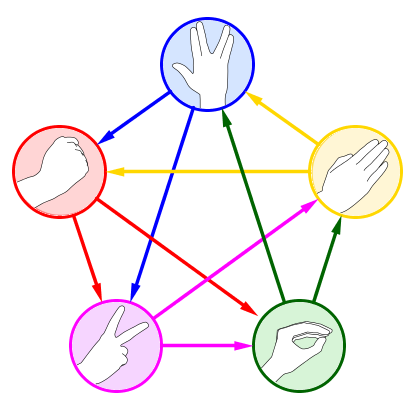
\includegraphics[width=4cm]{ressources/pfcls.png}
\end{center}
\end{frame}
\begin{frame}
    \frametitle{}

L'utilisateur peut connaître et donc décider de jouer à la variante du jeu contre la machine.
\begin{activite}
Modifier la fonction telle que sa \emph{signature} s'écrive \textbf{\texttt{choix\_machine(variante)}}. Le \emph{paramètre} \textbf{\texttt{variante}} sera un booléen. Si l'\emph{argument} passé lors de l'appel de la fonction est:
\begin{itemize}
    \item \textbf{\texttt{True}}: la fonction doit renvoyer un mot parmi les cinq de la variante,
    \item \textbf{\texttt{False:}} la fonction doit renvoyer un mot parmi les trois de la version classique.
\end{itemize}
\end{activite}

\end{frame}
\begin{frame}[fragile]
    \frametitle{Correction}
\begin{lstlisting}[language=Python , basicstyle=\ttfamily\small, xleftmargin=2em, xrightmargin=2em]
# La fonction possède un paramètre
def choix_machine(variante):
    if variante:
        valeur = randint(1, 5)        
    else:
        valeur = randint(1, 3)
        
    if valeur == 1:
        choix = "pierre"
    elif valeur == 2:
        choix = "feuille"
    elif valeur == 3:
        choix = "ciseaux"
    elif valeur == 4:
        choix = "lézard"
    else:
        choix = "Spock"
    return choix
\end{lstlisting}
\end{frame}
\begin{frame}[fragile]
    \frametitle{Correction}

\begin{center}
\begin{lstlisting}[language=Python , basicstyle=\ttfamily\small, xleftmargin=2em, xrightmargin=2em]
# Lors de l'appel de la fonction on lui passe un argument
machine = choix_machine(True)
\end{lstlisting}
\captionof{code}{Appel de la fonction pour jouer à la variante.}
\label{CODE}
\end{center}
\end{frame}
\subsection{Variables locales}
\begin{frame}[fragile]
    \frametitle{Variables locales}

\begin{center}
\begin{lstlisting}[language=Python , basicstyle=\ttfamily\small, xleftmargin=2em, xrightmargin=2em]
def choix_machine():
    valeur = randint(1, 3)
    if valeur == 1:
        choix = "pierre"
    elif valeur == 2:
        choix = "feuille"
    else:
        choix = "ciseaux"
    return choix
\end{lstlisting}
{\Large \href{https://pythontutor.com/visualize.html#code=from%20random%20import%20randint%0A%0Adef%20choix_machine%28%29%3A%0A%20%20%20%20valeur%20%3D%20randint%281,%203%29%0A%20%20%20%20if%20valeur%20%3D%3D%201%3A%0A%20%20%20%20%20%20%20%20choix%20%3D%20%22pierre%22%0A%20%20%20%20elif%20valeur%20%3D%3D%202%3A%0A%20%20%20%20%20%20%20%20choix%20%3D%20%22feuille%22%0A%20%20%20%20else%3A%0A%20%20%20%20%20%20%20%20choix%20%3D%20%22ciseaux%22%0A%20%20%20%20return%20choix%0A%0Amachine%20%3D%20choix_machine%28%29&cumulative=false&curInstr=0&heapPrimitives=nevernest&mode=display&origin=opt-frontend.js&py=3&rawInputLstJSON=%5B%5D&textReferences=false}{Visualisation}}
\end{center}

\end{frame}
\begin{frame}
    \frametitle{}

    \begin{itemize}
        \item<1-> Les variables \textbf{\texttt{valeur}} et \textbf{\texttt{choix}} sont \textbf{locales}.
        \item<2-> La fonction ne renvoie pas la variable \textbf{\texttt{choix}} mais le \textbf{contenu de cette variable}.
    \end{itemize}

\end{frame}
\section{Bonnes pratiques}
\begin{frame}[fragile]
    \frametitle{Bonnes pratiques}

\begin{center}
    \begin{lstlisting}[language=Python , basicstyle=\ttfamily\small, xleftmargin=2em, xrightmargin=2em]
def choix_machine(variante: bool) -> str:
    if variante:
        valeur = randint(1, 5)        
    else:
        valeur = randint(1, 3)
        
    if valeur == 1:
        choix = "pierre"
    elif valeur == 2:
        choix = "feuille"
    elif valeur == 3:
        choix = "ciseaux"
    elif valeur == 4:
        choix = "lézard"
    else:
        choix = "Spock"
    return choix
\end{lstlisting}    
\end{center}
\end{frame}
\begin{frame}
    \frametitle{}

    \begin{aretenir}[]
    On s'attachera à fournir un maximum d'informations dans la \textbf{signature} d'une fonction.
    \\ \centering \textbf{\texttt{choix\_machine(variante: bool) $\rightarrow$ str}}
    \end{aretenir}

\end{frame}
\begin{frame}[fragile]
    \frametitle{}

    \begin{center}
        \begin{lstlisting}[language=Python , basicstyle=\ttfamily\small, xleftmargin=2em, xrightmargin=2em]
def choix_machine(variante: bool) -> str:
    """
    Donne la proposition de la machine.

    Args:
        variante (booléen): choix de la variante

    Returns:
        str: renvoie le choix de la machine
    """
    if variante:
        ...
\end{lstlisting}    
    \end{center}   

\end{frame}
\begin{frame}
    \frametitle{}

\begin{aretenir}[]
\centering On fournira une \textbf{docstring} à chaque fonction.
\end{aretenir}

\end{frame}
\end{document}
